\documentclass[10pt,a4paper]{article}

\usepackage[T1]{fontenc}
\usepackage[utf8]{inputenc}
\usepackage{lmodern}
\usepackage[margin=1.8cm, top=1.6cm, bottom=1.8cm]{geometry}
\usepackage{microtype}
\usepackage{booktabs}
\usepackage{tabularx}
\usepackage{array}
\usepackage{xcolor}
\usepackage{tikz}
\usetikzlibrary{arrows.meta, positioning, calc, fit, backgrounds}
\tikzset{
  box/.style={draw=black!55, rounded corners=3pt, minimum height=0.8cm, minimum width=2.3cm, align=center,
    font=\footnotesize, fill=white},
  hot/.style={draw=restored, line width=0.9pt, fill=restored!8},
  flow/.style={-{Latex[length=2mm]}, black!60, line width=0.7pt},
  hotflow/.style={-{Latex[length=2mm]}, restored, line width=0.9pt},
  tag/.style={font=\scriptsize, text=quiet},
}
\usepackage{enumitem}
\usepackage{caption}
\usepackage{float}
\usepackage{titlesec}
\usepackage[hidelinks]{hyperref}

\definecolor{restored}{RGB}{37,99,235}
\definecolor{degraded}{RGB}{214,40,40}
\definecolor{kept}{RGB}{165,165,155}
\definecolor{band}{RGB}{236,236,234}
\definecolor{quiet}{RGB}{110,110,110}

\newcolumntype{L}{>{\raggedright\arraybackslash}X}
\renewcommand{\arraystretch}{1.3}
\setlength{\parskip}{0.65em}
\linespread{1.04}
\setlength{\parindent}{0pt}
\setlist{itemsep=0.35em, topsep=0.4em}
\captionsetup{font=small, labelfont=bf, skip=8pt}
\setlength{\abovecaptionskip}{8pt}
\titlespacing*{\section}{0pt}{1.7em}{0.7em}
\titlespacing*{\subsection}{0pt}{1.4em}{0.5em}
\setlength{\intextsep}{12pt}
\setlength{\textfloatsep}{14pt}
\setlength{\emergencystretch}{2em}

\begin{document}

\begin{center}
{\Large\bfseries Re-ranking RAG on the GDPR: Failure Modes and Analysis}\\[0.4em]
{\normalsize Shubhadeep Mandal \quad\textbar\quad 2025201056 \quad\textbar\quad 19 October 2026}
\end{center}
\vspace{0.6em}

\noindent Adding a cross-encoder re-ranker put the correct GDPR passage into the LLM's context for 6 of 13
hand-labelled stress-test questions where the bi-encoder alone missed it, and broke 1. It costs about 83\,ms per
query, under 1\% of end-to-end time.

\section*{Setup}

Both pipelines run over the GDPR (Regulation (EU) 2016/679, 88 pages), split into 305 chunks of 220 words with a
40-word overlap. The bi-encoder is \texttt{all-MiniLM-L6-v2} with a FAISS index, the cross-encoder
\texttt{ms-marco-MiniLM-L-6-v2}, and both pipelines answer with \texttt{gemini-3.7-flash}. The test set is 13
questions, each labelled with its gold chunk(s) and grouped by the failure it probes. Timings are averaged over 5
runs per query on a CUDA GPU.

\begin{figure}[!htbp]
\centering
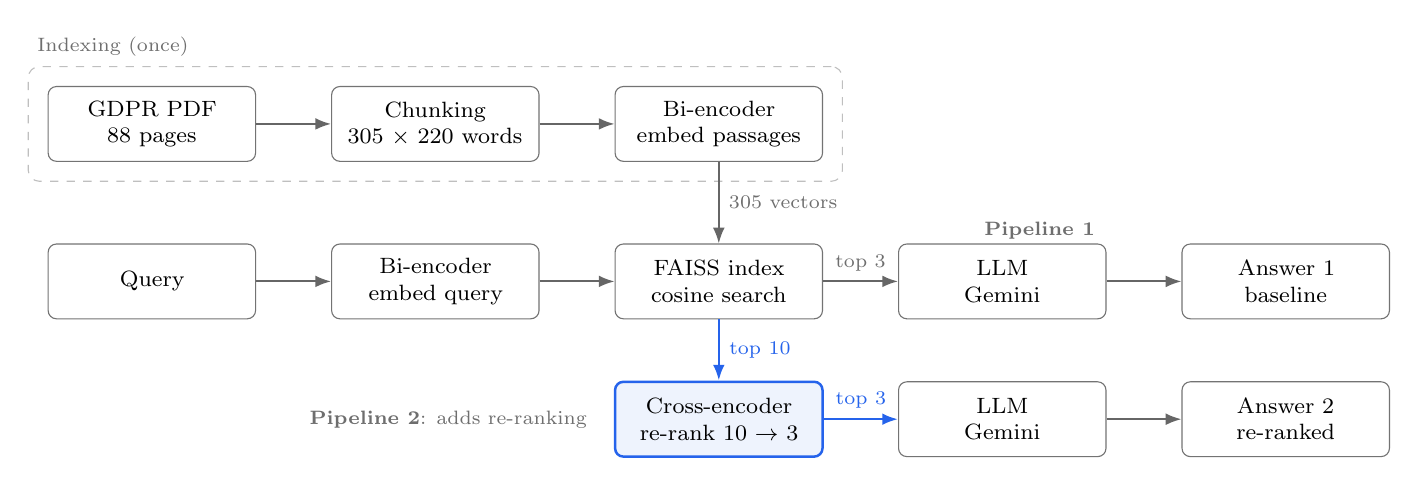
\begin{tikzpicture}
  \tikzset{cell/.style={box, minimum width=2.6cm, text width=2.4cm, minimum height=0.95cm}}
  % five evenly spaced columns, three rows
  \def\ca{1.3} \def\cb{4.9} \def\cc{8.5} \def\cd{12.1} \def\ce{15.7}

  % indexing, done once
  \node[cell] (pdf)   at (\ca, 0) {GDPR PDF\\88 pages};
  \node[cell] (chunk) at (\cb, 0) {Chunking\\305 $\times$ 220 words};
  \node[cell] (benc0) at (\cc, 0) {Bi-encoder\\embed passages};
  \draw[flow] (pdf) -- (chunk);
  \draw[flow] (chunk) -- (benc0);
  \begin{scope}[on background layer]
    \node[draw=black!25, dashed, rounded corners=4pt, inner sep=7pt, fit=(pdf)(benc0),
      label={[tag, anchor=south west]north west:Indexing (once)}] {};
  \end{scope}

  % query time, shared by both pipelines
  \node[cell] (query) at (\ca, -2.0) {Query};
  \node[cell] (benc)  at (\cb, -2.0) {Bi-encoder\\embed query};
  \node[cell] (faiss) at (\cc, -2.0) {FAISS index\\cosine search};
  \draw[flow] (query) -- (benc);
  \draw[flow] (benc) -- (faiss);
  \draw[flow] (benc0) -- node[tag, right] {305 vectors} (faiss);

  % Pipeline 1: straight on
  \node[cell] (llm1) at (\cd, -2.0) {LLM\\Gemini};
  \node[cell] (a1)   at (\ce, -2.0) {Answer 1\\baseline};
  \draw[flow] (faiss) -- node[tag, above] {top 3} (llm1);
  \draw[flow] (llm1) -- (a1);

  % Pipeline 2: one extra step
  \node[cell, hot] (cr) at (\cc, -3.75) {Cross-encoder\\re-rank 10 $\rightarrow$ 3};
  \node[cell] (llm2) at (\cd, -3.75) {LLM\\Gemini};
  \node[cell] (a2)   at (\ce, -3.75) {Answer 2\\re-ranked};
  \draw[hotflow] (faiss) -- node[tag, right, text=restored] {top 10} (cr);
  \draw[hotflow] (cr) -- node[tag, above, text=restored] {top 3} (llm2);
  \draw[flow] (llm2) -- (a2);

  % lane labels in the empty left cells
  \node[tag, anchor=east] at ({\cc-1.55}, -3.75) {\textbf{Pipeline 2}: adds re-ranking};
  \node[tag, anchor=east] at ({\cd+1.3}, -1.35) {\textbf{Pipeline 1}};
\end{tikzpicture}
\caption{The two pipelines share the index and the first-stage search. Pipeline 2 adds one step: the
cross-encoder re-scores the bi-encoder's top 10 and passes its own top 3 to the LLM.}
\end{figure}

% ─────────────────────────────────────────────────────────────────────────────
\section{Failure mode analysis}

Re-ranking restored the gold passage in every required category; one question got worse. Table~1 shows one
representative case per failure type. Five more (erasure, dismissal of the data protection officer (DPO), data
portability, child consent, a control) had the gold in the top 3 under both pipelines and are left out.

\begin{table}[!htbp]
\centering\scriptsize
\begin{tabularx}{\textwidth}{@{}p{1.3cm}>{\raggedright\arraybackslash}p{4.1cm}>{\raggedright\arraybackslash}p{3.1cm}L>{\raggedright\arraybackslash}p{1.25cm}@{}}
\toprule
\textbf{Category} & \textbf{Query} & \textbf{Gold passage (chunk)} & \textbf{Why the bi-encoder stumbles} & \textbf{Outcome} \\
\midrule
Keyword trap & Does a startup with 10 staff have to maintain records of processing? & Art.~30(5), ``fewer than 250 persons'' (193) & ``Records of processing'' matches Recital 82 word for word; the answer says ``250 persons'', never ``startup'' or ``staff'' & \textcolor{restored}{Restored} \\
Keyword trap & How long can personal data be stored? & Art.~5(1)(e), storage limitation (146) & Gold never enters the top 10, so the re-ranker has nothing to promote & Both miss \\
Exception & Must every company appoint a data protection officer? & Art.~37(1), when a DPO is mandatory (205) & Finds Art.~37(4), the general ``may designate'' rule, and misses the conditions & \textcolor{restored}{Restored} \\
Exception & Does a controller always have to notify affected individuals about a data breach? & Art.~34(3), when notice is not required (197, 198) & Gets the general duty (Recital 86) but not the ``except when'' list & \textcolor{restored}{Restored} \\
Negation & Is processing someone's religious beliefs or health information prohibited? & Art.~9(1), the prohibition (153) & ``Prohibited'' blurs with recitals on derogations; gold sits at rank 10 & \textcolor{restored}{Restored} \\
Buried & What is the maximum fine for breaching the basic principles of processing? & Art.~83(5), 20\,M EUR or 4\% (291, 292) & Returns the neighbouring 10\,M EUR\,/\,2\% tier, Art.~83(4) & \textcolor{restored}{Restored} \\
Degraded & Can the Commission ask the Board to examine a matter affecting more than one Member State? & Art.~64(2) (264) & Bi-encoder had it at rank 2; the cross-encoder pushed it to 8 & \textcolor{degraded}{Degraded} \\
\bottomrule
\end{tabularx}
\caption{Representative stress-test questions, one or two per failure type.}
\end{table}

\subsection*{Failure hunt and standard retrieval metrics}

To check that the hand-picked questions were not cherry-picked, \texttt{gemini-3.6-flash} wrote 100 more: an
ordinary question and a \textbf{wording trap} (borrowing a phrase from the most similar other passage) for each
of 50 passages. On ordinary questions re-ranking restored 8 and degraded 2; on wording traps it restored 2 and
degraded 5, because the cross-encoder can be pulled toward the passage the phrase came from. 30 of 100 were missed
by both pipelines: if the gold is not in the bi-encoder's top 10, re-ranking cannot help.

\begin{table}[!htbp]
\centering\small
\begin{tabular}{@{}lrrrr@{}}
\toprule
 & \multicolumn{2}{c}{\textbf{13 hand-labelled}} & \multicolumn{2}{c}{\textbf{100 generated}} \\
\cmidrule(lr){2-3}\cmidrule(l){4-5}
\textbf{Metric} & \textbf{Baseline} & \textbf{Re-ranked} & \textbf{Baseline} & \textbf{Re-ranked} \\
\midrule
Hit@1                                   & 0.23 & \textbf{0.46} & 0.34 & \textbf{0.42} \\
Hit@3 / Recall@3 (gold reaches the LLM) & 0.46 & \textbf{0.85} & 0.60 & \textbf{0.63} \\
Hit@10                                  & 0.92 & 0.92 & 0.77 & 0.77 \\
MRR@10                                  & 0.40 & \textbf{0.64} & 0.50 & \textbf{0.55} \\
Precision@3                             & 0.18 & \textbf{0.31} & 0.22 & \textbf{0.24} \\
nDCG@10                                 & 0.47 & \textbf{0.64} & 0.53 & \textbf{0.57} \\
\bottomrule
\end{tabular}
\caption{Retrieval metrics. Hit@10 cannot change: the re-ranker reorders the same 10 candidates.}
\end{table}

Hit@$k$ counts a hit when any gold chunk is in the top $k$; MRR uses the first gold chunk; Precision@3 and nDCG@10
use every gold chunk (binary relevance). Precision@3 stays low because most questions have only one gold chunk,
so 0.33 is its ceiling for them. The hand-labelled set was built to stress the
baseline, so the hunt's smaller gain (Hit@3 $+3$ points) is closer to everyday use. Answer-level metrics
(faithfulness, answer relevance) were not scored automatically; Section~3 compares answers by hand.

% ─────────────────────────────────────────────────────────────────────────────
\section{Architecture comparison}

A bi-encoder encodes the query and each passage separately and compares two vectors. A cross-encoder reads them
as one sequence, so every query token can attend to every passage token.

\begin{figure}[!htbp]
\centering
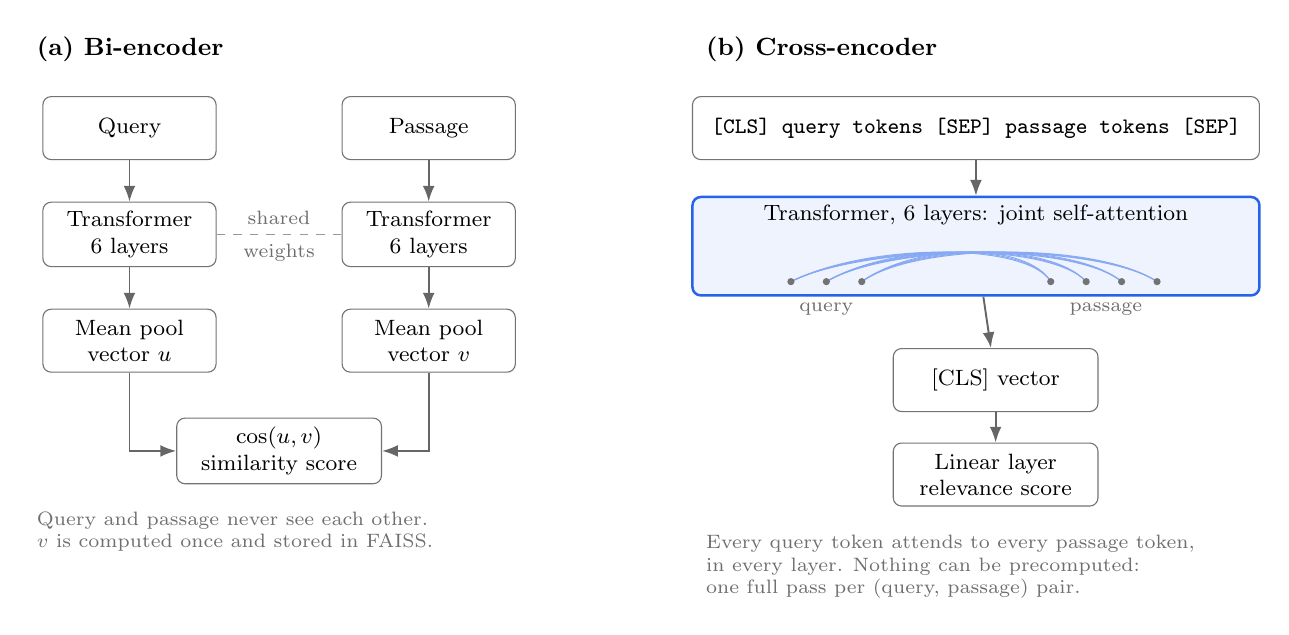
\begin{tikzpicture}
  % (a) bi-encoder
  \node[font=\small\bfseries, anchor=west] at (-0.1, 1.0) {(a) Bi-encoder};
  \node[box, minimum width=2.2cm] (q)  at (1.2, 0)    {Query};
  \node[box, minimum width=2.2cm] (p)  at (5.0, 0)    {Passage};
  \node[box, minimum width=2.2cm] (eq) at (1.2, -1.35) {Transformer\\6 layers};
  \node[box, minimum width=2.2cm] (ep) at (5.0, -1.35) {Transformer\\6 layers};
  \node[box, minimum width=2.2cm] (u)  at (1.2, -2.7) {Mean pool\\vector $u$};
  \node[box, minimum width=2.2cm] (v)  at (5.0, -2.7) {Mean pool\\vector $v$};
  \node[box, minimum width=2.6cm] (cos) at (3.1, -4.1) {$\cos(u, v)$\\similarity score};
  \draw[flow] (q) -- (eq); \draw[flow] (eq) -- (u);
  \draw[flow] (p) -- (ep); \draw[flow] (ep) -- (v);
  \draw[black!40, dashed] (eq) -- node[tag, above] {shared} node[tag, below] {weights} (ep);
  \draw[flow] (u.south) |- (cos.west);
  \draw[flow] (v.south) |- (cos.east);
  \node[tag, align=left, anchor=north west] at (-0.1, -4.75)
    {Query and passage never see each other.\\$v$ is computed once and stored in FAISS.};

  % (b) cross-encoder
  \node[font=\small\bfseries, anchor=west] at (8.4, 1.0) {(b) Cross-encoder};
  \node[box, minimum width=7.2cm, font=\footnotesize\ttfamily] (in) at (11.95, 0)
    {[CLS] query tokens [SEP] passage tokens [SEP]};
  \node[box, hot, minimum width=7.2cm, minimum height=1.25cm] (tr) at (11.95, -1.5) {};
  \node[font=\footnotesize, anchor=north] at (tr.north) {Transformer, 6 layers: joint self-attention};
  \foreach \a in {0,1,2} {
    \foreach \b in {0,1,2,3} {
      \draw[restored!55, line width=0.35pt] ({9.6+\a*0.45}, -1.95) .. controls ({10.6+\a*0.3}, -1.45) and ({12.6+\b*0.3}, -1.45) .. ({12.9+\b*0.45}, -1.95);
    }
  }
  \foreach \a in {0,1,2} \fill[black!55] ({9.6+\a*0.45}, -1.95) circle (1.3pt);
  \foreach \b in {0,1,2,3} \fill[black!55] ({12.9+\b*0.45}, -1.95) circle (1.3pt);
  \node[tag] at (10.05, -2.3) {query};
  \node[tag] at (13.6, -2.3) {passage};
  \node[box, minimum width=2.6cm] (cls) at (12.2, -3.2) {[CLS] vector};
  \node[box, minimum width=2.6cm] (sc)  at (12.2, -4.4) {Linear layer\\relevance score};
  \draw[flow] (in) -- (tr);
  \draw[flow] (tr) -- (cls);
  \draw[flow] (cls) -- (sc);
  \node[tag, align=left, anchor=north west] at (8.4, -5.05)
    {Every query token attends to every passage token,\\in every layer. Nothing can be precomputed:\\one full pass per (query, passage) pair.};
\end{tikzpicture}
\caption{(a) The bi-encoder compresses each text into one 384-d vector on its own, so relevance is a single dot
product. (b) The cross-encoder reads the pair as one sequence and outputs a relevance score directly.}
\end{figure}

The bi-encoder answers ``is this passage about the same thing?''; the cross-encoder answers ``does this passage
answer this question?''. Squeezing a passage into one vector means a passage that shares the query's words or
topic scores close to the right one, and ``not'' or ``except'' barely moves the vector. That is why the
cross-encoder pulled Art.~9(1) up from rank 10: it is the sentence that says processing is \emph{prohibited},
while the recitals ranked above it only discuss the topic. The price is speed: the bi-encoder's passage vectors
are built once, while the cross-encoder must run one full pass for every candidate at query time.

% ─────────────────────────────────────────────────────────────────────────────
\section{Qualitative and rank shift analysis}

\begin{figure}[!htbp]
\centering
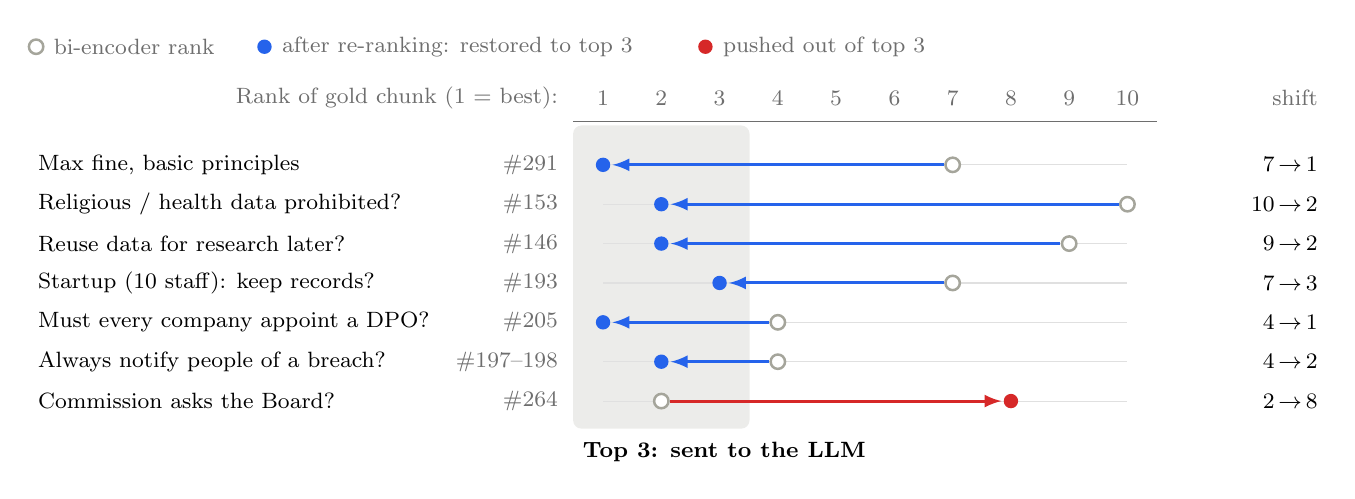
\begin{tikzpicture}[x=1cm, y=1cm, font=\footnotesize]
  % top-3 band
  \fill[band, rounded corners=3pt] ({7.3-0.38}, 0.35) rectangle ({7.3+2*0.74+0.38}, -3.5);
  % rank axis
  \foreach \k in {1,...,10} \node[quiet] at ({7.3+(\k-1)*0.74}, 0.7) {\k};
  \draw[quiet] ({7.3-0.38}, 0.4) -- ({7.3+9*0.74+0.38}, 0.4);
  \node[quiet, anchor=east] at (16.5, 0.7) {shift};
  \node[quiet, anchor=east] at (6.85, 0.7) {Rank of gold chunk (1 = best):};
  % rows: index / label / chunk / bi / ce / colour
  \foreach \i/\q/\c/\b/\e/\col in {
      0/{Max fine, basic principles}/\#291/7/1/restored,
      1/{Religious / health data prohibited?}/\#153/10/2/restored,
      2/{Reuse data for research later?}/\#146/9/2/restored,
      3/{Startup (10 staff): keep records?}/\#193/7/3/restored,
      4/{Must every company appoint a DPO?}/\#205/4/1/restored,
      5/{Always notify people of a breach?}/\#197--198/4/2/restored,
      6/{Commission asks the Board?}/\#264/2/8/degraded} {
    \pgfmathsetmacro{\y}{-0.5*\i-0.15}
    \pgfmathsetmacro{\xb}{7.3+(\b-1)*0.74}
    \pgfmathsetmacro{\xe}{7.3+(\e-1)*0.74}
    \draw[black!12] (7.3, \y) -- ({7.3+9*0.74}, \y);
    \node[anchor=west] at (0, \y) {\q};
    \node[anchor=east, quiet] at (6.85, \y) {\c};
    \draw[\col, line width=1.1pt, -{latex}, shorten <=3.2pt, shorten >=3.4pt] (\xb, \y) -- (\xe, \y);
    \draw[kept, line width=0.9pt, fill=white] (\xb, \y) circle (2.6pt);
    \fill[\col] (\xe, \y) circle (2.6pt);
    \node[anchor=east] at (16.5, \y) {\b\,$\rightarrow$\,\e};
  }
  \node[font=\footnotesize\bfseries, anchor=west] at ({7.3-0.38}, -3.8) {Top 3: sent to the LLM};
  % legend
  \begin{scope}[shift={(0,1.35)}]
    \draw[kept, line width=0.9pt, fill=white] (0.1,0) circle (2.6pt); \node[anchor=west, quiet] at (0.2,0) {bi-encoder rank};
    \fill[restored] (3.0,0) circle (2.6pt); \node[anchor=west, quiet] at (3.1,0) {after re-ranking: restored to top 3};
    \fill[degraded] (8.6,0) circle (2.6pt); \node[anchor=west, quiet] at (8.7,0) {pushed out of top 3};
  \end{scope}
\end{tikzpicture}
\caption{Re-ranking lifted the gold chunk into the top 3 for 6 questions; one fell from rank 2 to 8. The biggest
lifts came from deep in the list: Art.~9(1) rose 10\,$\rightarrow$\,2 and the 20\,M EUR fine tier
7\,$\rightarrow$\,1.}
\end{figure}

The baseline never invented a rule outright. Its failures were quieter: it said the context did not cover the
question, stated a general rule without its exception, or quoted the wrong tier, each time because the chunk with
the deciding clause sat outside the top 3. The research and breach questions failed like the DPO question (rule
without its exception), so Table~3 omits them.

\begin{table}[!htbp]
\centering\scriptsize
\begin{tabularx}{\textwidth}{@{}>{\raggedright\arraybackslash}p{3.0cm}LL>{\raggedright\arraybackslash}p{2.7cm}@{}}
\toprule
\textbf{Query} & \textbf{Answer 1 (baseline)} & \textbf{Answer 2 (re-ranked)} & \textbf{Baseline failure} \\
\midrule
Startup with 10 staff: records of processing? & ``Not possible to answer''; quotes only Recital 82's general duty & Generally exempt under Art.~30(5) (fewer than 250 persons), unless the processing is risky, not occasional or covers special categories & Omitted the deciding exemption; no answer \\
Must every company appoint a DPO? & No; cites only Art.~37(4) ``may designate'' & No; lists the three mandatory cases of Art.~37(1)(a)--(c) & Omitted the conditions that make it mandatory \\
Religious beliefs or health data prohibited? & Says the context does not list them as prohibited & Yes; Art.~9(1) prohibits it, with the Art.~9(2) exceptions & Misstated the rule: denied a prohibition that exists \\
Maximum fine for breaching basic principles? & ``Not explicitly stated''; gives the 10\,M EUR\,/\,2\% tier of Art.~83(4) & 20\,M EUR or 4\% of worldwide turnover, Art.~83(5)(a) & Wrong tier on offer; no answer \\
Commission asks the Board? \emph{(degraded)} & Yes; quotes Art.~64(2) & ``Not explicitly stated''; text cuts off & Reverse: re-ranking dropped the gold chunk \\
\bottomrule
\end{tabularx}
\caption{Answer 1 vs Answer 2 for representative queries.}
\end{table}

Because the prompt tells the model to answer only from the context, a dropped chunk produces a cautious ``not
stated'' rather than a confident error, in either pipeline.

% ─────────────────────────────────────────────────────────────────────────────
\section{Latency profiling}

Re-ranking makes retrieval $7.5\times$ slower (12.7\,$\rightarrow$\,95.4\,ms) but adds only 0.9\% to the
end-to-end time, because LLM generation takes about 9.2\,s either way.

\begin{table}[!htbp]
\centering\small
\begin{tabular}{@{}lrr@{}}
\toprule
\textbf{Stage (mean, ms)} & \textbf{Pipeline 1 (baseline)} & \textbf{Pipeline 2 (re-ranked)} \\
\midrule
Bi-encoder: embed query + FAISS search & 12.73 (top 3) & 12.73 (top 10) \\
Cross-encoder: score 10 pairs & --- & 82.62 \\
\textbf{Retrieval total} & \textbf{12.73} & \textbf{95.35} \\
LLM generation (\texttt{gemini-3.7-flash}) & 9,223.5 & 9,223.5 \\
\textbf{End-to-end} & \textbf{9,236.23} & \textbf{9,318.85} \\
\bottomrule
\end{tabular}
\end{table}

Medians are within 1\,ms of the means. Generation time ranged from 5.5 to 18.2\,s per answer, driven by answer
length rather than the pipeline. On the CPU (8 threads) the 10-pair re-rank takes about 1\,s, still small next to
generation.

% ─────────────────────────────────────────────────────────────────────────────
\section{Scaling: why not cross-encode everything?}

A cross-encoder over the whole collection costs one transformer pass per passage for every query, and nothing can
be computed ahead of time. Scanning this 305-chunk regulation takes 2.65\,s; a million passages would take 2.4
hours per question.

\begin{table}[!htbp]
\centering\small
\begin{tabular}{@{}rrr@{}}
\toprule
\textbf{Collection size (chunks)} & \textbf{Cross-encoder full scan} & \textbf{Two-stage: re-rank top 10} \\
\midrule
305 (this GDPR, measured) & 2.65\,s & 82.62\,ms \\
100,000 & 870\,s (14.5\,min) & 82.62\,ms \\
1,000,000 & 8,700\,s (2.4\,h) & 82.62\,ms \\
10,000,000 & 87,001\,s (24.2\,h) & 82.62\,ms \\
\bottomrule
\end{tabular}
\end{table}

\begin{itemize}
  \item \textbf{No precomputation.} The score depends on query and passage together, so nothing can be cached or
    indexed. Bi-encoder vectors are built once; a FAISS search stays in milliseconds at millions of vectors.
  \item \textbf{Cost grows with the collection.} A full scan is linear in $N$ (8.7\,ms per pair); the two-stage
    design costs a fixed $k = 10$ pairs.
  \item \textbf{Precision only matters at the top.} The bi-encoder only has to get the answer into the top 10
    (recall); the cross-encoder spends its expensive attention ordering those 10 (precision).
\end{itemize}

The catch is that the re-ranker can only promote what the bi-encoder found (30 of 100 hunt questions missed in
both). Section~6 widens the first stage with BM25 to target those, at a cost that grows with $k$, not $N$.

\section{Follow-up: hybrid retrieval and query rewriting}

\textbf{Hybrid.} BM25 (over the same chunks, numbers kept as tokens) and the bi-encoder each return their top 20;
Reciprocal Rank Fusion ($\sum 1/(60 + \mathrm{rank})$) merges the lists and the fused top 10 go to the same
cross-encoder, so re-ranking still costs 10 pairs. Fusion adds 1.3\,ms per query.
\textbf{HyDE.} The local Qwen3.5-4B (Q4\_K\_M, temperature 0) writes one or two sentences of the passage that
would answer the question, in the regulation's wording; the bi-encoder's ranking for that passage is fused as a
third list and BM25 searches question and passage together. The cross-encoder still scores the original question.

\begin{table}[!htbp]
\centering\small
\begin{tabular}{@{}lrrrrrr@{}}
\toprule
 & \multicolumn{3}{c}{\textbf{13 hand-labelled}} & \multicolumn{3}{c}{\textbf{100 generated}} \\
\cmidrule(lr){2-4}\cmidrule(l){5-7}
\textbf{After re-ranking} & \textbf{Dense} & \textbf{Hybrid} & \textbf{+\,HyDE} & \textbf{Dense} & \textbf{Hybrid} & \textbf{+\,HyDE} \\
\midrule
Hit@1   & \textbf{0.46} & 0.38 & \textbf{0.46} & 0.42 & 0.43 & \textbf{0.44} \\
Hit@3   & \textbf{0.85} & 0.77 & 0.69 & 0.63 & 0.72 & \textbf{0.73} \\
Hit@10  & 0.92 & 0.92 & 0.85 & 0.77 & \textbf{0.93} & 0.92 \\
MRR@10  & \textbf{0.64} & 0.59 & 0.59 & 0.55 & \textbf{0.61} & \textbf{0.61} \\
Added latency & -- & 1.3\,ms & 5.6\,s & -- & 1.3\,ms & 5.6\,s \\
\bottomrule
\end{tabular}
\caption{Dense is the report's Pipeline 2 and reproduces Table~2. Hybrid and HyDE change only the 10 candidates.}
\end{table}

On the hunt, hybrid brought 16 of the 23 questions the bi-encoder missed into the top 10 and lost none; the gold
reached the LLM for 12 more questions and 3 fewer. To check that this reaches the answers, the 16 questions whose
top 3 changed were answered by Qwen from both top 3s. All 12 gains became correct answers (dense: 10 ``not in the
context'', one wrong, one incomplete). Of the 4 losses, one stayed correct, one became an abstention, one partly
right, and one wrong: the startup question, where BM25 matches ``records of processing'' in Art.~30(1) and pushes
the Art.~30(5) exemption (``fewer than 250 persons'') from rank 3 to 5, and the model answers that a 10-person
startup must keep records. The hand-labelled set was written to defeat keyword overlap, so its small loss is
expected; the hunt is closer to everyday questions. On a second document, the Constitution of India (124 hunt
questions), hybrid helps more evenly: re-ranked Hit@3 0.67 to 0.75 and Hit@10 0.77 to 0.91, with 12 questions
restored and 2 degraded, and its 12-question case study gains one and loses none. Answering the 15 changed
questions with Qwen3.5-4B (fp16 on a Kaggle T4, same prompt), hybrid turned 9 wrong or ``not in the context''
answers into correct ones; 4 were correct either way, because another chunk repeated the fact; one became an
abstention (a cut-off date the dense top 3 had); one question was too garbled to grade. Hybrid produced no
confident wrong answer, where dense gave five (for example citing Art.~98 for a rule in Art.~187).

HyDE adds almost nothing over hybrid on the hunt (Hit@3 $+1$ point; 6 restored, 5 degraded) and loses a question on
the hand-labelled set, for 5.6\,s of generation per query. A 4B model's guess at the law is often wrong in the
detail that matters: for the startup question it invented the Art.~30 criteria instead of the 250-person
threshold, so the rewrite pulls toward the general rule. Hybrid is worth keeping; HyDE with a small model is not.

\section{Follow-up: structure-aware chunking}

The 220-word windows cut wherever the count falls, often mid-article. The alternative makes each provision
(an Article or Recital of the GDPR, a ``21.~Title.---'' article of the Constitution) a unit: small units are
packed together and long ones split at their numbered paragraphs, both up to the same 220 words, so only the
boundaries change. A third variant embeds and re-ranks each chunk under its heading (``Article 30 Records of
processing activities''). Gold chunk ids depend on the chunking, so gold is located in the text instead: each
question's snippet is found inside its saved gold chunks, and under any chunking a chunk is gold if it holds at
least half of that span. On the windows this returns the saved labels for 106 of 113 GDPR questions; the other
7 add the neighbouring window that shares the snippet through the overlap.

\begin{table}[!htbp]
\centering\small
\begin{tabular}{@{}llrrrrr@{}}
\toprule
 & & \multicolumn{2}{c}{\textbf{GDPR (100)}} & \multicolumn{2}{c}{\textbf{Constitution (113)}} & \\
\cmidrule(lr){3-4}\cmidrule(lr){5-6}
\textbf{Chunking} & \textbf{Retrieval} & \textbf{Hit@3} & \textbf{MRR@10} & \textbf{Hit@3} & \textbf{MRR@10} & \textbf{Words to LLM} \\
\midrule
Window (current)    & dense  & 0.63 & 0.55 & 0.73 & 0.64 & 660 \\
Window              & hybrid & 0.72 & 0.61 & \textbf{0.82} & 0.70 & 660 \\
Structure           & dense  & 0.71 & 0.61 & 0.65 & 0.60 & 490 \\
Structure           & hybrid & 0.76 & 0.65 & 0.81 & \textbf{0.73} & 490 \\
Structure + heading & dense  & 0.76 & 0.64 & 0.68 & 0.59 & 495 \\
Structure + heading & hybrid & \textbf{0.79} & \textbf{0.69} & 0.79 & 0.71 & 500 \\
\bottomrule
\end{tabular}
\caption{Failure-hunt questions after re-ranking. Words to LLM: mean length of the top 3 that reach the model.
Window + dense reproduces Table~2 (GDPR); its Constitution figures differ from above because 11 questions without
a locatable snippet are left out.}
\end{table}

On the GDPR, structure-aware chunks help with either retriever: with dense retrieval, Hit@3 rises 8 points
(structure) or 13 (structure + heading; 18 questions restored, 5 degraded), and structure + heading + hybrid is the best configuration measured (Hit@3 0.79, MRR 0.69),
while sending the model a quarter less text, because structure chunks average 151 words against 220. Headings add
3 to 5 points; the GDPR windows had none. On the Constitution the picture is mixed: with dense retrieval alone
structure chunks are worse (Hit@3 0.73 to 0.65, Hit@10 0.81 to 0.70), and with hybrid they tie on Hit@3 but rank
the gold first more often (Hit@1 0.56 to 0.62). Its windows were already searched under their article labels, so
headings add nothing there. The 13 and 12 hand-labelled questions move by one question either way and are not
informative here. Structure-aware chunking is worth it for a cleanly structured regulation, not as a blanket
default.

\section*{Conclusion}

On a legal text where the deciding clause often sits beside a general rule (an exemption, a higher fine tier, a
prohibition), a cross-encoder re-ranker is worth its 83\,ms: it turned 6 incomplete or wrong answers into correct,
cited ones. It is not free of failure: wording traps can mislead it, and it cannot recover passages the bi-encoder
never retrieves. Fusing BM25 into the first stage fixes most of those for 1.3\,ms (hunt Hit@10 0.77 to 0.93, Hit@3
0.63 to 0.72); rewriting the query with a small local model does not pay for its 5.6\,s. Cutting chunks at
article boundaries, with headings, lifts the GDPR further (Hit@3 0.79) on a quarter less context, but did not help
the Constitution of India, so it suits documents whose structure parses cleanly.

\section*{Code}

Notebook, saved results, this report and the live app:
\url{https://github.com/Seronic2001/retrieve-ten-keep-three}

\end{document}
